\documentclass[11pt]{article}%设置文档类型{article}和字体大小{11pt}，适配本地字体

\usepackage[a4paper]{geometry}%页面布局，纸张大小[a4paper]
\geometry{left=2.0cm,right=2.0cm,top=2.5cm,bottom=2.5cm}%页面边距
\usepackage[UTF8]{ctex}%latex支持中文宏包
\usepackage{amsmath, amsfonts, amssymb, amsthm}%数学公式环境、数学字体、数学字体扩展包、定理环境
\usepackage{bm,mathtools}%数学粗体、amsmath扩展包
\usepackage{graphicx}%插入和管理图片
\usepackage[graphicx]{realboxes}%创建和管理盒子（装有文本和图形）
\usepackage{algorithm,algorithmicx}%支持伪代码宏包
\usepackage[noend]{algpseudocode}%支持伪代码宏包
\usepackage{fancyhdr}%定制页眉和页脚
\setlength{\headheight}{13.6pt}%避免页眉高度警告
\pagestyle{fancy}
\fancyhf{} % 清空默认的页眉和页脚
\fancyhead[L]{\kaishu 中国科学院大学}
\fancyhead[C]{林俊杰2023K8009916012}
\fancyhead[R]{\kaishu}
\fancyfoot[C]{\thepage}
\usepackage{booktabs}%美化表格宏包
\usepackage{caption}%定制图表标题宏包
\usepackage{xcolor}%切换字体颜色
\usepackage{placeins}%控制浮动体位置
\usepackage{cleveref}%智能引用
\crefname{figure}{图}{figures}
\Crefname{figure}{Figure}{Figures}
\crefname{table}{表}{tables}
\Crefname{table}{Table}{Tables}
\usepackage{tikz} % 绘图宏包
\usetikzlibrary{arrows.meta, positioning, calc, shapes, fit, decorations.pathreplacing} % 加载绘图库   

%数学环境计数器
\newcounter{counter_exm}\setcounter{counter_exm}{1}
%\newcounter{counter_thm}\setcounter{counter_thm}{1}
%\newcounter{counter_lma}\setcounter{counter_lma}{1}
%\newcounter{counter_dft}\setcounter{counter_dft}{1}
%\newcounter{counter_clm}\setcounter{counter_clm}{1}
%\newcounter{counter_cly}\setcounter{counter_cly}{1}

%图标随章节计数{章节.张数}
\counterwithin{figure}{section}
\counterwithin{table}{section}

\newtheorem{theorem}{{\hskip 1.7em \bf 定理}}
\newtheorem{lemma}[theorem]{\hskip 1.7em 引理}
\newtheorem{proposition}[theorem]{Proposition}
\newtheorem{claim}[theorem]{\hskip 1.7em 命题}
\newtheorem{corollary}[theorem]{\hskip 1.7em 推论}
\newtheorem{definition}[theorem]{\hskip 1.7em 定义}

\renewcommand{\emph}[1]{{\kaishu #1}}
\newcommand{\articlename}{反向传播}

\newenvironment{solution}{{\noindent\hskip 2em \bf 解 \quad}}{\par}
\newenvironment{example}{{\noindent\hskip 2em \bf 例 \arabic{counter_exm}\quad}}{\addtocounter{counter_exm}{1}\par}
\newenvironment{concept}[1]{{\bf #1\quad} \begin{kaishu}}{\end{kaishu}\par}
\renewenvironment{proof}{{\noindent\hskip 2em \bf 证明 \quad}}{\hfill$\qed$\par}

\begin{document}
    \begin{center}
        \LARGE \bf \articlename
    \end{center}

    \section{单层神经网络}
    
    单层神经网络可以看作是一个简单的线性变换后接一个激活函数：
    \begin{equation*}
        L(x) = f(W \cdot x + b)
    \end{equation*}

    \begin{figure}[H]
        \centering
        \begin{tikzpicture}[
            >=Stealth, line width=0.8pt,
            % ---- 预定义样式 ----
            box/.style = {draw, rectangle, minimum size=0.8cm, fill=white, inner sep=0pt},
            tallbox/.style = {draw, rectangle, minimum width=0.8cm, minimum height=2.4cm, fill=white, inner sep=0pt},
            sum/.style = {draw, circle, inner sep=0pt, minimum size=0.6cm},
            mybrace/.style = {decorate, decoration={brace, amplitude=6pt}},
            small brace/.style = {decorate, decoration={brace, amplitude=4pt}}
        ]

        % ===================== 左侧区域 =====================
        % 灰色矩形 p（中心默认为 (0,0)）
        \node[draw, rectangle, fill=gray!80, minimum width=0.6cm, minimum height=2.8cm] (p) {};
        \node (num1) at ($(p.east)+(0.5,-0.65)$) {1};   % 数字“1”

        % 小括号：输入标记
        \draw[small brace] ($(p.north west)+(0,0.35)$) -- ($(p.north east)+(0,0.35)$)
            node[midway, above=4pt] {输入};

        % ===================== 右侧区域 =====================
        % W 和 b 盒子（相对于 p.east 偏移）
        \node[box] (W) at ($(p.east)+(1.9,0.65)$) {$W$};
        \node[below=2pt of W, inner sep=0pt] {\scriptsize $S \times R$};

        \node[box] (b) at ($(p.east)+(1.9,-0.65)$) {$b$};
        \node[below=2pt of b, inner sep=0pt] {\scriptsize $S \times 1$};

        % 加号（W 和 b 右侧的中间位置）
        \coordinate (mid) at ($(W)!0.5!(b)$);
        \node[sum] (plus) at ($(mid)+(1.6,0)$) {\large $+$};

        % f 高矩形（加号右侧）
        \node[tallbox] (f) at ($(plus)+(1.7,0)$) {$f$};

        % ---- 连线 ----
        \draw[->] (p.east |- W.west) -- (W.west)
            node[midway, above=1pt] {$x$}
            node[midway, below=1pt] {\scriptsize $R \times 1$};
        \draw[->] (num1.east) -- (b.west);
        \draw[->] (W.east) -- (plus);
        \draw[->] (b.east) -- (plus);
        \draw[->] (plus.east) -- (f.west)
            node[midway, above=1pt] {$z$}
            node[midway, below=1pt] {\scriptsize $S \times 1$};
        % 输出箭头（从 f 右上角引出）
        \draw[->] ([yshift=-0.6cm]f.north east) -- ++(1.4,0)
            node[midway, above=1pt] {$a$}
            node[midway, below=1pt] {\scriptsize $S \times 1$};

        % 在大括号前先定义一个水平高度（基于 f 的顶部上移 0.55cm）
        \coordinate (braceY) at ($(f.north)+(0,0.55cm)$);

        % 画大括号：左边 x 取 W.west 偏左 0.1，右边 x 取 f.east 偏右 0.1，y 统一用 braceY
        \draw[mybrace]
            ($(braceY -| W.west)+(-0.1,0)$) --
            ($(braceY -| f.east)+(0.1,0)$)
            node[midway, above=6pt] {具有$S$个神经元的层};

        \end{tikzpicture}
        \caption{单层神经网络}
    \end{figure}

    \section{多层感知机 (MLP)}

    多层感知机就是多个单层网络的叠加（复合）：
    \begin{equation*}
        MLP(x) = L^L \circ L^{L-1} \circ \dots \circ L^1(x)
    \end{equation*}
    其中每一层 $L^l(\cdot) = f^l(W^l \cdot + b^l)$。
    将每层的“线性部分”和“非线性部分”分开看：
    \begin{equation*}
    \underbrace{z^{l} = W^{l} a^{l-1} + b^{l}}_{\text{线性：参数都在这里}}
    \qquad\quad
    \underbrace{a^{l} = f(z^{l})}_{\text{非线性：无参数}}
    \end{equation*}

    \section{反向传播 (BP) 算法推导}

    反向传播旨在迭代地计算梯度。
    \begin{figure}[H]
        \centering
        \resizebox{\textwidth}{!}{
        \begin{tikzpicture}[>=Stealth, node distance=1cm, 
            box/.style={draw, rectangle, minimum height=2.8cm, minimum width=1.8cm, dashed}]
            
            \node (x) {$x$};
            \node[right=1.0cm of x] (z1) {$z^1$};
            \node[above=0.6cm of z1] (W1) {$W^1$};
            \node[right=0.6cm of z1] (a1) {$a^1$};
            \node[below=0.6cm of z1] (b1) {$b^1$};
            \node[right=1.0cm of a1] (z2) {$z^2$};
            \node[above=0.6cm of z2] (W2) {$W^2$};
            \node[right=0.6cm of z2] (a2) {$a^2$};
            \node[below=0.6cm of z2] (b2) {$b^2$};
            \node[right=1.0cm of a2] (dots) {$\dots$};
            \node[right=0.6cm of dots] (al_m) {$a^{l-1}$};
            \node[right=1.0cm of al_m] (zl) {$z^l$};
            \node[above=0.6cm of zl] (Wl) {$W^l$};
            \node[right=0.6cm of zl] (al) {$a^l$};
            \node[below=0.6cm of zl] (bl) {$b^l$};
            \node[right=1.0cm of al] (dots2) {$\dots$};
            \node[right=0.6cm of dots2] (aL) {$a^L$};
            \node[right=1.0cm of aL] (L) {$L$};
            
            \draw[->] (x) -- (z1); \draw[->] (W1) -- (z1); \draw[->] (z1) -- (a1); \draw[->] (b1) -- (z1);
            \draw[->] (a1) -- (z2); \draw[->] (W2) -- (z2); \draw[->] (z2) -- (a2); \draw[->] (b2) -- (z2);
            \draw[->] (a2) -- (dots); \draw[->] (dots) -- (al_m);
            \draw[->] (al_m) -- (zl); \draw[->] (Wl) -- (zl); \draw[->] (zl) -- (al); \draw[->] (bl) -- (zl);
            \draw[->] (al) -- (dots2); \draw[->] (dots2) -- (aL); \draw[->] (aL) -- (L);

            \node[box, fit=(W1) (z1) (b1) (a1), label=below:{$L^1$}] {};
            \node[box, fit=(W2) (z2) (b2) (a2), label=below:{$L^2$}] {};
            \node[box, fit=(Wl) (zl) (bl) (al), label=below:{$L^l$}] {};
        \end{tikzpicture}
        }
        \caption{MLP 中的变量依赖关系}
    \end{figure}

    我们的\textbf{目标}是计算 $\frac{\partial L}{\partial W^l}$ 与 $\frac{\partial L}{\partial b^{l}}$，对每一层 $l$。
    但\textbf{困难}是 $W^{l}$ 离 $L$ 隔着许多层，如果要直接对它求偏导，需要把链式法则一路推到底。
    逐个层地展开，最终会得到一个非常长的链式乘积，计算量大且容易出错。
    所以我们需要利用一些中间变量来\textbf{分解}这个长链式，迭代地计算梯度。

    \subsection{参数梯度的分解}
    注意到一个自然的\textbf{简化}：
    所有从 $W^{l}$ 和 $b^{l}$ 出发去往 $L$ 的路径，总是可以分解为先到达 $z^{l}$，再从 $z^{l}$ 到 $L$。所以只要拿到误差项
    \begin{equation*}
    \delta^{l} = \frac{\partial L}{\partial z^{l}}
    \end{equation*}
    剩下的就是 $z^{l}$ 怎么显式依赖 $W^{l}$ 和 $b^{l}$，那一步是平凡的（线性）。这就把原来的“长链式”切成两段，
    于是计算过程重新组织为：先算每一层的 $\delta^{l}$，再用它合成参数梯度。

    \begin{figure}[H]
        \centering
        \resizebox{0.8\textwidth}{!}{
        \begin{tikzpicture}[>=Stealth, node distance=1cm, 
            box/.style={draw, rectangle, minimum height=2.8cm, minimum width=1.8cm, dashed}]
                        
            \node (al_m) {$a^{l-1}$};
            \node[right=1.0cm of al_m] (zl) {$z^l$};
            \node[above=0.6cm of zl] (Wl) {$W^l$};
            \node[right=0.6cm of zl] (al) {$a^l$};
            \node[below=0.6cm of zl] (bl) {$b^l$};
            \node[right=1.0cm of al] (dots2) {$\dots$};
            \node[right=0.6cm of dots2] (aL) {$a^L$};
            \node[right=1.0cm of aL] (L) {$L$};
            
            \draw[->] (al_m) -- (zl);
            \draw[->] (zl) -- (al);
            \draw[->] (al) -- (dots2);
            \draw[->] (dots2) -- (aL);
            \draw[->] (aL) -- (L);

            % ===== W^l <-> z^l 双向直线(平行不重叠) =====
            \draw[->] ($(Wl.south)-(2pt,0)$) -- ($(zl.north)-(2pt,0)$);
            \draw[->, red] ($(zl.north)+(2pt,0)$) -- ($(Wl.south)+(2pt,0)$);
            
            % ===== b^l <-> z^l 双向直线(平行不重叠) =====
            \draw[->] ($(bl.north)-(2pt,0)$) -- ($(zl.south)-(2pt,0)$);
            \draw[->, red] ($(zl.south)+(2pt,0)$) -- ($(bl.north)+(2pt,0)$);

            % ===== L -> z^l 红色曲线(从西侧进入，避免与上方箭头相交) =====
            \draw[->, red, out=135, in=45, looseness=0.8] (L.north west) to (zl.north east);
        \end{tikzpicture}
        }
        \caption{参数梯度分解}
    \end{figure}
 
    接下来，我们使用\textbf{爱因斯坦求和约定}，假设已经得到第 $l$ 层的误差项 $\delta^l$，计算该层参数梯度具体的分量：
    \begin{align*}
        \frac{\partial L}{\partial W_{ij}^l} &= \frac{\partial L}{\partial z_i^l} \frac{\partial z_i^l}{\partial W_{ij}^l} = \delta_i^l a_j^{l-1} \\
        \frac{\partial L}{\partial b_i^l} &= \frac{\partial L}{\partial z_i^l} \frac{\partial z_i^l}{\partial b_i^l} \phantom{al} = \delta_i^l
    \end{align*}

    \subsection{误差项的递推公式 ($\delta^l \to \delta^{l-1}$)}
    想要从后往前地计算梯度，我们还需要误差项的递推公式，这是 BP 算法的核心。
    \begin{figure}[H]
        \centering
        \resizebox{0.8\textwidth}{!}{
        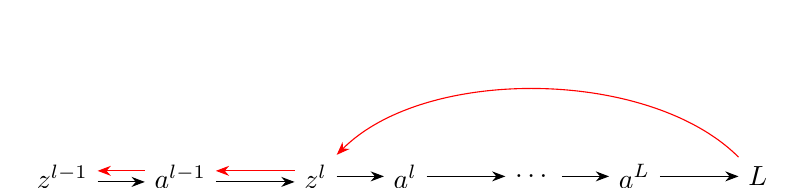
\begin{tikzpicture}[>=Stealth, node distance=1cm, 
            box/.style={draw, rectangle, minimum height=2.8cm, minimum width=1.8cm, dashed}]
            
            \node(zl_m) {$z^{l-1}$};
            \node[right=0.6cm of zl_m] (al_m) {$a^{l-1}$};
            \node[right=1.0cm of al_m] (zl) {$z^l$};
            \node[right=0.6cm of zl] (al) {$a^l$};
            \node[right=1.0cm of al] (dots2) {$\dots$};
            \node[right=0.6cm of dots2] (aL) {$a^L$};
            \node[right=1.0cm of aL] (L) {$L$};
            
            \draw[->] (zl) -- (al);
            \draw[->] (al) -- (dots2);
            \draw[->] (dots2) -- (aL);
            \draw[->] (aL) -- (L);
            \draw[->] ($(zl_m.east)-(0,2pt)$) -- ($(al_m.west)-(0,2pt)$);
            \draw[->, red] ($(al_m.west)+(0,2pt)$) -- ($(zl_m.east)+(0,2pt)$);
            \draw[->] ($(al_m.east)-(0,2pt)$) -- ($(zl.west)-(0,2pt)$);
            \draw[->, red] ($(zl.west)+(0,2pt)$) -- ($(al_m.east)+(0,2pt)$);
            \draw[->, red, out=135, in=45, looseness=0.8] (L.north west) to (zl.north east);
        \end{tikzpicture}
        }
        \caption{误差项递推分解}
    \end{figure}

    \begin{equation*}
        \delta_i^{l-1} = \frac{\partial L}{\partial z_i^{l-1}} = \frac{\partial L}{\partial z_j^l} \frac{\partial z_j^l}{\partial a_k^{l-1}} \frac{\partial a_k^{l-1}}{\partial z_i^{l-1}} = \delta_j^l W_{jk}^l \frac{\partial a_k^{l-1}}{\partial z_i^{l-1}}
    \end{equation*}

    \begin{itemize}
        \item \textbf{分量独立情况}（若 $a_k = f(z_k)$）：
        每个激活值仅取决于对应的净输入。
        \begin{equation*}
            \delta_i^{l-1} = \delta_j^l W_{ji}^l \odot f'(z_i^{l-1})
        \end{equation*}
        \item \textbf{分量相关情况}（如 Softmax）：
        \begin{equation*}
            \delta_i^{l-1} = \delta_j^l W_{jk}^l F_{ki}^{l-1}
        \end{equation*}
        其中 $F_{ki}^{l-1}$ 是激活函数的雅可比矩阵。此时 $j, k$ 为\emph{哑变量}。
    \end{itemize}

    \subsection{迭代的起点：$\delta^L$}
    最后，我们给这个递推公式一个“首项”。
    \begin{figure}[H]
        \centering
        \resizebox{0.4\textwidth}{!}{
        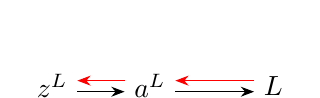
\begin{tikzpicture}[>=Stealth, node distance=1cm, 
            box/.style={draw, rectangle, minimum height=2.8cm, minimum width=1.8cm, dashed}]
            
            \node(zL) {$z^L$};
            \node[right=0.6cm of zL] (aL) {$a^L$};
            \node[right=1.0cm of aL] (L) {$L$};
            
            \draw[->] ($(zL.east)-(0,2pt)$) -- ($(aL.west)-(0,2pt)$);
            \draw[->, red] ($(aL.west)+(0,2pt)$) -- ($(zL.east)+(0,2pt)$);
            \draw[->] ($(aL.east)-(0,2pt)$) -- ($(L.west)-(0,2pt)$);
            \draw[->, red] ($(L.west)+(0,2pt)$) -- ($(aL.east)+(0,2pt)$);
        \end{tikzpicture}
        }
        \caption{$\delta^L$ 的计算}
    \end{figure}

    \begin{equation*}
        \delta_i^L = \frac{\partial L}{\partial a_j^L} \frac{\partial a_j^L}{\partial z_i^L}
    \end{equation*}

    \begin{itemize}
        \item \textbf{分量不独立}：
        \begin{equation*}
            \delta_i^L = \frac{\partial L}{\partial a_j^L} F_{ji}^L
        \end{equation*}
        \item \textbf{分量独立}：
        \begin{equation*}
            \delta_i^L = \frac{\partial L}{\partial a_i^L} \odot f'(z_i^L)
        \end{equation*}
    \end{itemize}

    \section{对照总结表}

    \begin{table}[H]
        \centering
        \begin{tabular}{lcc}
            \toprule
            物理量 & 分量形式 (Einstein Convention) & 矩阵形式 \\
            \midrule
            输出层误差 (独立) & $\delta_i^L = \frac{\partial L}{\partial a_i^L} \odot f'(z_i^L)$ & $\delta^L = \frac{\partial L}{\partial a^L} \odot f'(z^L)$ \\
            输出层误差 (通用) & $\delta_i^L = \frac{\partial L}{\partial a_j^L} F_{ji}^L$ & $\delta^L = (F^L)^T \frac{\partial L}{\partial a^L}$ \\
            权重梯度 & $\frac{\partial L}{\partial W_{ij}^l} = \delta_i^l a_j^{l-1}$ & $\frac{\partial L}{\partial W^l} = \delta^l (a^{l-1})^T$ \\
            偏置梯度 & $\frac{\partial L}{\partial b_i^l} = \delta_i^l$ & $\frac{\partial L}{\partial b^l} = \delta^l$ \\
            误差递推 (独立) & $\delta_i^{l-1} = \delta_j^l W_{ji}^l f'(z_i^{l-1})$ & $\delta^{l-1} = (W^l)^T \delta^l \odot f'(z^{l-1})$ \\
            误差递推 (通用) & $\delta_i^{l-1} = \delta_j^l W_{jk}^l F_{ki}^{l-1}$ & $\delta^{l-1} = (F^{l-1})^T (W^l)^T \delta^l$ \\
            \bottomrule
        \end{tabular}
        \caption{分量形式与矩阵形式对照}
    \end{table}

    分量形式的好处就是转置位置一目了然（看哑指标在哪一位），且能无痛推广到张量（卷积、batch 维度），不必纠结“先转置还是先 reshape”。

    \section{总结}

    MLP 的反向传播算法的流程可以总结为：
    \begin{enumerate}
        \item 从输出层开始，计算 $\delta^L$。
        \item 使用 $\delta^l$ 计算每层的参数梯度 $\frac{\partial L}{\partial W^l}$ 和 $\frac{\partial L}{\partial b^l}$。
        \item 迭代地使用递推公式计算 $\delta^{l-1}$。
        \item 重复步骤 2 和 3，直到计算到输入层。
    \end{enumerate}

    \section{引申：从反向传播到自动微分}

    我们并不满足只能在 MLP 上进行反向传播，接下来讨论如何在一般结构的网络上进行参数梯度的计算。

    \subsection{我们到底遇到了什么困难？}

    \textbf{情形 1：} 
    $$
    y = \theta_1^2 + \theta_2^2 + \dots + \theta_n^2
    $$

    \begin{figure}[H]
        \centering
        \resizebox{0.4\textwidth}{!}{
        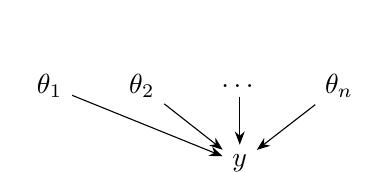
\begin{tikzpicture}[>=Stealth, node distance=1cm]
            
            \node (theta1) {$\theta_1$};
            \node[right=0.6cm of theta1] (theta2) {$\theta_2$};
            \node[right=0.6cm of theta2] (dots) {$\dots$};
            \node[right=0.6cm of dots] (thetan) {$\theta_n$};
            \node[below=0.6cm of dots] (y) {$y$};
            
            \draw[->] (theta1) -- (y);
            \draw[->] (theta2) -- (y);
            \draw[->] (dots) -- (y);
            \draw[->] (thetan) -- (y);
        \end{tikzpicture}
        }
        \caption{情形 1 的计算图}
    \end{figure}

    此时
    $$
    \frac{\partial y}{\partial \theta_i} = 2\theta_i
    $$
    每一个分量可以对 $y$ 偏导一次直接得到，每次求导的计算是不可避免的。

    \textbf{情形 2：}
    \begin{align*}
    y &= \theta_1^2 + \varphi_1 \\
    \theta_1 &= \theta_2^2 + \varphi_2 \\
    \theta_2 &= \theta_3^2 + \varphi_3 \\
    &\dots \\
    \theta_{n-1} &= \theta_n^2
    \end{align*}

    \begin{figure}[H]
        \centering
        \resizebox{0.5\textwidth}{!}{
        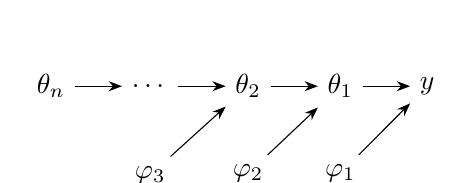
\begin{tikzpicture}[>=Stealth, node distance=1cm]
            
            \node (thetan) {$\theta_n$};
            \node[right=0.6cm of thetan] (dots) {$\dots$};
            \node[right=0.6cm of dots] (theta2) {$\theta_2$};
            \node[right=0.6cm of theta2] (theta1) {$\theta_1$};
            \node[right=0.6cm of theta1] (y) {$y$};
            
            \node[below=0.75cm of dots] (varphi_aux) {$\varphi_3$};
            \node[below=0.6cm of theta2] (varphi2) {$\varphi_2$};
            \node[below=0.6cm of theta1] (varphi1) {$\varphi_1$};
            
            \draw[->] (varphi1) -- (y);
            \draw[->] (theta1) -- (y);
            \draw[->] (theta2) -- (theta1);
            \draw[->] (dots) -- (theta2);
            \draw[->] (thetan) -- (dots);
            \draw[->] (varphi2) -- (theta1);
            \draw[->] (varphi_aux) -- (theta2);
        \end{tikzpicture}
        }
        \caption{情形 2 的计算图}
    \end{figure}

    通过链式法则计算：
    \begin{align*}
        \frac{\partial y}{\partial \varphi_1} &= 1 \\
        \frac{\partial y}{\partial \varphi_2} &= \frac{\partial y}{\partial \theta_1} \cdot \frac{\partial \theta_1}{\partial \varphi_2} = 2\theta_1 \cdot 1 \\
        &\vdots \\
        \frac{\partial y}{\partial \theta_n} &= \frac{\partial y}{\partial \theta_1} \dots \frac{\partial \theta_{n-1}}{\partial \theta_n} = 2\theta_1 \cdot 2\theta_2 \dots 2\theta_n
    \end{align*}
    可以发现，在计算过程中出现了很多重复项，导致计算量巨大。

    \subsection{两者计算开销有本质区别！}

    假设：对 $y=f(x)$，计算 $\frac{\partial y}{\partial x}$ 需要 1 个单位时间。

    \begin{itemize}
        \item \textbf{情形 1：} 计算 $\frac{\partial y}{\partial \theta}$ 的所有分量需要 $n$ 个单位时间，平均每个分量 1 单位时间。
        \item \textbf{情形 2：} 计算 $\frac{\partial y}{\partial \theta_i}$ 的第 $i$ 个分量需要使用链式法则，计算 $i$ 次偏导数。计算 $n$ 个偏导数总共需要 $\frac{n(n+1)}{2}$ 单位时间，平均每个变量需 $\frac{n+1}{2}$ 单位时间。时间线性增长远大于常数。
    \end{itemize}

    在普通的梯度计算中，依赖链的长度越长，重复计算的次数就越多，导致计算效率急剧下降。但是现代神经网络的计算图非常复杂，依赖链无可避免的非常长，如果不加以优化，计算梯度的效率将会非常低下。

    \textbf{如何避免？} 谜底就在谜面上：\textbf{用笔记本记下已经计算好的中间量，下次需要时直接取用即可}（类似斐波那契数列的递归优化）。

    \subsection{反向传播的推导}

    反向传播算法的核心思想就是利用动态规划的思想，迭代地计算每个节点的梯度，并将其存储起来，以避免重复计算。
    如果要计算某个节点 $v$ 的梯度 $\frac{\partial L}{\partial v}$，
    我们先计算它的所有直接后继节点 $v'$ 的梯度 $\frac{\partial L}{\partial v'}$，然后利用链式法则将它们组合起来： 
    \begin{equation*}
        \frac{\partial L}{\partial v} = \sum_{v' \in \text{succ}(v)} \frac{\partial L}{\partial v'} \cdot \frac{\partial v'}{\partial v}
    \end{equation*}
    
    我们可以用计算图直观地理解这个过程：
    计算图中的任意节点 $v$ 代表梯度 $\frac{\partial L}{\partial v}$，
    每个边代表一个局部梯度 $\frac{\partial v'}{\partial v}$。
    通过从输出层 $L$ 开始，沿着计算图逆向传播，每经过一条边，
    我们就将当前节点的梯度“乘”以该边的局部梯度 $ \frac{\partial v'}{\partial v}$，
    并将结果累加到前驱节点的梯度上。该前驱节点的梯度等于所有后继分支路径上所得梯度之和。

    计算某个节点的梯度之前，必须先计算它的所有后继节点的梯度，因此反向传播的计算顺序是按照计算图的逆拓扑排序进行的。

    \subsection{与正向计算的联系}

    在正向计算中，对于某个节点 $v$，我们要先计算它的所有前驱节点的值，然后才能计算 $v$ 的值。节点的计算顺序对应计算图的拓扑排序。
    在反向传播中，对于某个节点 $v$，我们要先计算它的所有后继节点的梯度，然后才能计算 $v$ 的梯度。节点的计算顺序对应计算图的逆拓扑排序。
    由于每个拓扑排序都有一个对应的逆拓扑排序，因此可以将正向计算的计算过程反向遍历一次，就可以得到反向传播的计算顺序。

    \subsection{自动微分的过程}

    结合前向计算和反向传播，我们可以构建出自动微分程序的整体流程。
    \begin{enumerate}
        \item \textbf{前向计算}：按照计算图的拓扑排序，从输入节点开始，逐层计算每个节点的值，并将其存储起来。
        \item \textbf{反向传播}：按照计算图的逆拓扑排序，从输出节点 $L$ 开始，逐层计算每个节点的梯度，并将其存储起来。
        \item \textbf{参数更新}：使用计算得到的梯度来更新模型参数，例如通过梯度下降算法。
    \end{enumerate}

    在这个过程中，前向计算和反向传播是紧密结合的，前向计算为反向传播提供了必要的中间值，而反向传播则利用这些中间值高效地计算梯度，从而实现了自动微分的功能。

    在构建一个自动微分程序时，我们需要设计一个数据结构来表示计算图中的节点和边，
    并实现前向计算和反向传播的算法。通常，节点会包含一个值和一个梯度，
    以及指向其前驱节点和后继节点的指针。
    边会定义如何用前驱节点的值计算后继节点，同时定义如何将后继节点的梯度“乘”以局部梯度来更新前驱节点的梯度。
\end{document}